% Assurance Lifecycle Flowchart - v6 vertical phases, horizontal flows
% Portrait-friendly layout

\documentclass[tikz,border=15pt]{standalone}
\usepackage{tikz}
\usetikzlibrary{shapes.geometric, arrows.meta, positioning, fit, backgrounds, calc}

\begin{document}

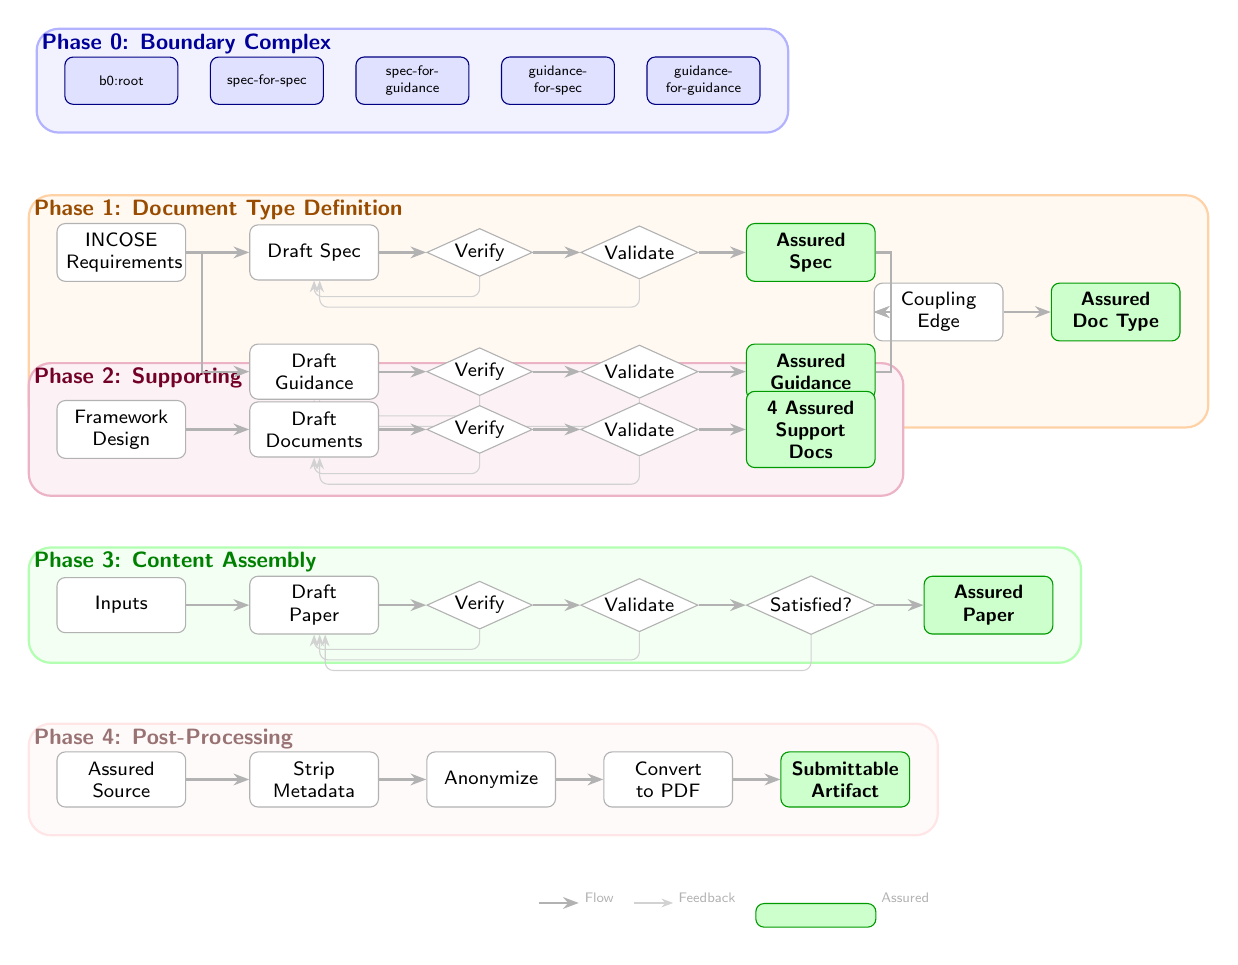
\begin{tikzpicture}[
    % Global settings
    font=\sffamily\small,
    % Box styles
    process/.style={
        rectangle, 
        draw=gray!60,
        fill=white,
        rounded corners=3pt,
        minimum height=0.7cm,
        minimum width=1.6cm,
        text centered,
        font=\sffamily\scriptsize,
        text width=1.4cm,
        align=center
    },
    decision/.style={
        diamond, 
        draw=gray!60,
        fill=white,
        aspect=2.2,
        minimum width=1.2cm,
        text centered,
        font=\sffamily\scriptsize,
        inner sep=1pt
    },
    assured/.style={
        process,
        fill=green!20,
        draw=green!60!black,
        font=\sffamily\scriptsize\bfseries
    },
    foundation/.style={
        rectangle,
        draw=blue!50!black,
        fill=blue!12,
        rounded corners=3pt,
        minimum width=1.4cm,
        minimum height=0.6cm,
        text centered,
        font=\sffamily\tiny,
        text width=1.2cm,
        align=center
    },
    % Arrow styles
    arrow/.style={-{Stealth[length=2mm]}, thick, gray!60},
    feedback/.style={-{Stealth[length=1.5mm]}, gray!35, rounded corners=3pt},
    % Phase box styles
    phasebox/.style={
        rounded corners=8pt,
        inner sep=10pt,
        thick
    },
    % Phase label style
    phaselabel/.style={
        font=\sffamily\footnotesize\bfseries,
        anchor=north west,
        inner sep=0pt
    }
]

% ===========================================
% PHASE 0: Boundary Complex
% ===========================================
\node[foundation] (ROOT) {b0:root};
\node[foundation, right=0.4cm of ROOT] (SS) {spec-for-spec};
\node[foundation, right=0.4cm of SS] (SG) {spec-for-guidance};
\node[foundation, right=0.4cm of SG] (GS) {guidance-for-spec};
\node[foundation, right=0.4cm of GS] (GG) {guidance-for-guidance};

\begin{scope}[on background layer]
    \node[phasebox, fill=blue!5, draw=blue!30,
          fit=(ROOT)(SS)(SG)(GS)(GG)] (P0) {};
    \node[phaselabel, blue!60!black] at ([xshift=2pt, yshift=-2pt]P0.north west) {Phase 0: Boundary Complex};
\end{scope}

% ===========================================
% PHASE 1: Document Type Definition
% Row 1: Spec path
% Row 2: Guidance path
% Then merge to Coupling → Assured Type
% ===========================================

% Starting point
\node[process, below=1.5cm of ROOT] (PM) {INCOSE\\Requirements};

% Spec row (top)
\node[process, right=0.8cm of PM] (DS) {Draft Spec};
\node[decision, right=0.6cm of DS] (VS) {Verify};
\node[decision, right=0.6cm of VS] (VaS) {Validate};
\node[assured, right=0.6cm of VaS] (AS) {Assured\\Spec};

% Guidance row (below spec row)
\node[process, below=0.8cm of DS] (DG) {Draft Guidance};
\node[decision, right=0.6cm of DG] (VG) {Verify};
\node[decision, right=0.6cm of VG] (VaG) {Validate};
\node[assured, right=0.6cm of VaG] (AG) {Assured\\Guidance};

% Merge point
\node[process, right=0.8cm of $(AS)!0.5!(AG)$] (CE) {Coupling\\Edge};
\node[assured, right=0.6cm of CE] (ADT) {Assured\\Doc Type};

% Phase 1 arrows
\draw[arrow] (PM.east) -- ++(0.2,0) |- (DS.west);
\draw[arrow] (PM.east) -- ++(0.2,0) |- (DG.west);
\draw[arrow] (DS) -- (VS);
\draw[arrow] (VS) -- (VaS);
\draw[arrow] (VaS) -- (AS);
\draw[arrow] (DG) -- (VG);
\draw[arrow] (VG) -- (VaG);
\draw[arrow] (VaG) -- (AG);
\draw[arrow] (AS.east) -- ++(0.2,0) |- (CE.west);
\draw[arrow] (AG.east) -- ++(0.2,0) |- (CE.west);
\draw[arrow] (CE) -- (ADT);

% Feedback loops (below each row)
\draw[feedback] (VS.south) -- ++(0,-0.25) -| (DS.south);
\draw[feedback] (VaS.south) -- ++(0,-0.35) -| ([xshift=2pt]DS.south);
\draw[feedback] (VG.south) -- ++(0,-0.25) -| (DG.south);
\draw[feedback] (VaG.south) -- ++(0,-0.35) -| ([xshift=2pt]DG.south);

\begin{scope}[on background layer]
    \node[phasebox, fill=orange!5, draw=orange!35,
          fit=(PM)(DS)(DG)(VS)(VG)(VaS)(VaG)(AS)(AG)(CE)(ADT)] (P1) {};
    \node[phaselabel, orange!60!black] at ([xshift=2pt, yshift=-2pt]P1.north west) {Phase 1: Document Type Definition};
\end{scope}

% ===========================================
% PHASE 2: Supporting Documents
% ===========================================
\node[process, below=1.5cm of PM] (IC) {Framework\\Design};
\node[process, right=0.8cm of IC] (DA) {Draft\\Documents};
\node[decision, right=0.6cm of DA] (VAr) {Verify};
\node[decision, right=0.6cm of VAr] (VaAr) {Validate};
\node[assured, right=0.6cm of VaAr] (AAr) {4 Assured\\Support Docs};

\draw[arrow] (IC) -- (DA);
\draw[arrow] (DA) -- (VAr);
\draw[arrow] (VAr) -- (VaAr);
\draw[arrow] (VaAr) -- (AAr);

% Feedback (below)
\draw[feedback] (VAr.south) -- ++(0,-0.25) -| (DA.south);
\draw[feedback] (VaAr.south) -- ++(0,-0.35) -| ([xshift=2pt]DA.south);

\begin{scope}[on background layer]
    \node[phasebox, fill=purple!5, draw=purple!30,
          fit=(IC)(DA)(VAr)(VaAr)(AAr)] (P2) {};
    \node[phaselabel, purple!60!black] at ([xshift=2pt, yshift=-2pt]P2.north west) {Phase 2: Supporting Documents};
\end{scope}

% ===========================================
% PHASE 3: Content Assembly
% ===========================================
\node[process, below=1.5cm of IC] (INPUTS) {Inputs};
\node[process, right=0.8cm of INPUTS] (DP) {Draft\\Paper};
\node[decision, right=0.6cm of DP] (VC) {Verify};
\node[decision, right=0.6cm of VC] (VaC) {Validate};
\node[decision, right=0.6cm of VaC] (SAT) {Satisfied?};
\node[assured, right=0.6cm of SAT] (AC) {Assured\\Paper};

\draw[arrow] (INPUTS) -- (DP);
\draw[arrow] (DP) -- (VC);
\draw[arrow] (VC) -- (VaC);
\draw[arrow] (VaC) -- (SAT);
\draw[arrow] (SAT) -- (AC);

% Feedback (below)
\draw[feedback] (VC.south) -- ++(0,-0.25) -| (DP.south);
\draw[feedback] (VaC.south) -- ++(0,-0.35) -| ([xshift=2pt]DP.south);
\draw[feedback] (SAT.south) -- ++(0,-0.45) -| ([xshift=4pt]DP.south);

\begin{scope}[on background layer]
    \node[phasebox, fill=green!5, draw=green!30,
          fit=(INPUTS)(DP)(VC)(VaC)(SAT)(AC)] (P3) {};
    \node[phaselabel, green!50!black] at ([xshift=2pt, yshift=-2pt]P3.north west) {Phase 3: Content Assembly};
\end{scope}

% ===========================================
% PHASE 4: Post-Processing
% ===========================================
\node[process, below=1.5cm of INPUTS] (AC2) {Assured\\Source};
\node[process, right=0.8cm of AC2] (STRIP) {Strip\\Metadata};
\node[process, right=0.6cm of STRIP] (ANON) {Anonymize};
\node[process, right=0.6cm of ANON] (PDF) {Convert\\to PDF};
\node[assured, right=0.6cm of PDF] (SUB) {Submittable\\Artifact};

\draw[arrow] (AC2) -- (STRIP);
\draw[arrow] (STRIP) -- (ANON);
\draw[arrow] (ANON) -- (PDF);
\draw[arrow] (PDF) -- (SUB);

\begin{scope}[on background layer]
    \node[phasebox, fill=pink!8, draw=pink!40,
          fit=(AC2)(STRIP)(ANON)(PDF)(SUB)] (P4) {};
    \node[phaselabel, pink!60!black] at ([xshift=2pt, yshift=-2pt]P4.north west) {Phase 4: Post-Processing};
\end{scope}

% ===========================================
% Legend - bottom right
% ===========================================
\node[anchor=north east, font=\sffamily\tiny, gray!60] 
    at ([yshift=-0.6cm]P4.south east) {
    \tikz[baseline]{\draw[arrow] (0,0) -- (0.5,0);} Flow \quad
    \tikz[baseline]{\draw[feedback] (0,0) -- (0.5,0);} Feedback \quad
    \tikz[baseline]{\node[assured, minimum width=0.7cm, minimum height=0.3cm, font=\tiny] {};} Assured
};

\end{tikzpicture}

\end{document}